\documentclass{article}
\usepackage[utf8]{inputenc}

% Tables
% Use Roman numerals for tables
% https://tex.stackexchange.com/a/226029
\usepackage[labelsep=period]{caption}
\captionsetup[table]{name=Table}
\renewcommand{\thetable}{\Roman{table}}
% \usepackage{multirow}

\usepackage{pdflscape}

% units
% \SI{X}{\UNIT} will write the value X with units \UNIT. 
% eg. \SI{30}{\celsius}
\usepackage{siunitx} 

\usepackage{graphicx}
\graphicspath{ {./images/} }

\usepackage{todonotes}
\newcommand{\tino}[1]{\todo[inline,color=purple!40]{Tino: #1}}
\newcommand{\fbp}[1]{\todo[inline,color=orange!40]{Ferran: #1}}
\newcommand{\summary}[1]{\todo[inline,caption={},color=yellow!40]{Summary: \\ #1}}

\newcommand{\ssr}[1]{{\textbf{\textcolor{blue}{Shashank: #1}}}}

\usepackage[normalem]{ulem}

\setlength{\textheight}{8.4in}
\setlength{\topmargin}{0.1in}
\setlength{\headheight}{0.2in}
\setlength{\headsep}{0.1in}
\setlength{\oddsidemargin}{0in}
\setlength{\textwidth}{6.5in}

\title{Knees in lithium-ion battery lifetime}
\author{To do}
\date{}

\begin{document}
\maketitle

**PREVIOUS DRAFT IS NOW IN main\_old\_experiment\_then\_model.tex**

\section{Introduction}

Lithium-ion batteries will continue to play a critical role in decarbonization via their use in electric vehicle and stationary energy storage applications. One of the most challenging requirements for these demanding use cases is long lifetime, with typical warranties of X years for electric vehicles and X years for grid storage[lit values?]. Battery lifetime requirements will only become more demanding as “million-mile batteries” become the expectation for next-generation electric vehicles. Furthermore, as concerns around battery mining, manufacturing, and disposal increase, improving battery lifetime is a straightforward way to reduce the environmental impact of the lithium-ion battery lifecycle. Thus, understanding and improving the lifetime of lithium-ion batteries is a critical research direction.

Lithium ion batteries often exhibit one of three degradation patterns: linear, sublinear, or superlinear aging (Figure 1). In laboratory settings (i.e., single-cell testing using battery cyclers), degradation is typically presented as capacity or energy vs. cycle number. Cells often degrade linearly[] or sublinearly[]. Sublinear degradation is often attributed to side reactions such as the solid-electrolyte interphase (SEI) growth, which grows approximately[] (but not exactly[]) with the square root of time or cycle number due to its self-passivsting nature. While this type of degradation is largely unavoidable, the decelerating degradation rate is a fortunate property for long-lifetime applications. However, superlinear battery degradation is also often observed (Figure 1c). This type of degradation goes by many names in the battery literature, including “knee”, “rollover failure”, “sudden death”, “accelerated aging”, “nonlinear aging”, etc; we use the term “knee” in the remainder of this work. Avoiding this type of degradation is critical to ensure long lifetimes in the field. However, despite many experimental and modeling reports on this topic, a comprehensive understanding of knees is lacking, likely due to the variety and complexity of proposed mechanisms.

In this review, we survey the literature and critically examine both experimental and modeling work on the subject of knees. We first review methods to define the knee point. We then classify experimental observations of knees in the literature; broadly, all cells with differences in knee behavior can be attributed to either differences in design, differences in usage conditions, or cell-to-cell/testing variation. Building on these Finally, we briefly discuss physics-driven and data-driven approaches to knee prediction, practical guidelines for avoiding knees, and suggested future work on this topic. This review can serve both academic and industrial efforts to understand and improve battery lifetime.

\section{Defining the knee point}

Figure 2.

\section{Pathways for knee points}

\subsection{Thermodynamic lithium plating}
\paragraph{LLI}
Li inventory loss due to thermodynamic Li plating may occur whenever there is not enough negative electrode capacity to store all of the available lithium during charging.
\paragraph{LAM_{deNE}}
Surface layer growth ...
Delamination ...
Dry out...


\subsection{Kinetic lithium plating}
\paragraph{LLI}
Li plating may also occur heterogeneously, when the local Li+ potential exceeds the nucleation barrier, leading to direct plating even in cases where the average graphite to Li potential would not lead to plating. Direct heterogenous Li plating can be driven by a wide range of design and usage conditions; the prototypical usage case leading to Li plating is high charging rates at low temperature \cite{waldmann_temperature_2014, petzl_lithium_2015}. Note that there are no consistent quantitative values for ‘high’ charging rate or ‘low’ temperature, as plating will occur whenever the local potential exceeds the energy barrier for Li nucleation. Thus, plating may be observed even at fairly normal test conditions, such as 1C CC charging near room temperature \cite{waldmann_optimization_2015,burns_-situ_2015}. Increasing temperature and cell design may allow for much more rapid charging before Li plating and knee-over is observed; Lewerenz et al cycled cells at rates up to 8C, observing no obvious knee-over up to 4C, though microstructural evidence of Li plating was found even at 1C \cite{lewerenz_systematic_2017}. The onset of direct lithium plating is also very sensitive to the charging protocol, with many studies demonstrating that informed design of charge protocols can substantially extend cell lifetime by preventing direct lithium plating \cite{waldmann_optimization_2015,schindler_fast_2018}.
Design conditions - anode porosity, electrode channels, particle sizes / distribution….? Experimental evidence? Lots of modeling work on microstructure being done at NREL.

\paragraph{ORI}
...

\paragraph{LAM_{deNE}}
Localized loss of negative electrode active material sites can cause heterogenous Li plating by impeding the transport of Li, locally increasing the overpotential and eventually causing plating. There are several mechanisms that may lead to LAMdeNE: surface layer growth, delamination, and electrolyte dry-out.

Surface layer growth on the negative electrode may impede Li transport into the negative electrode during charging. This surface layer has been often observed during accelerated aging of LIBs, and is most commonly attributed to Mn or Fe dissolution from the cathode and electrolyte salt decomposition \cite{lewerenz_post-mortem_2017,lewerenz_systematic_2017,zhu_investigation_2021,stiaszny_electrochemical_2014,rahe_nanoscale_2019,keil_linear_2019,sarasketa-zabala_understanding_2015, willenberg_high-precision_2020}. Lewerenz et al documented surface layer growth very thoroughly, finding that increasing C-rate and larger depth-of-discharge could lead to earlier onset of a knee, which was correlated with the presence of a thick surface layer on cells that contained knees; cells without knees also contained obvious surface layers, but with lower surface coverage and less thickness \cite{lewerenz_post-mortem_2017,lewerenz_systematic_2017}. These surface layers sometimes seem to lead directly to localized lithium plating, with lithium observed on top of the layer \cite{zhu_investigation_2021}.

Delamination may also lead to inaccessible negative electrode material, which can potentially cause lithium plating and knee-onset. Willenberg et al conclusively observed delamination induced knee-onset in cylindrical cells; delamination was caused due to mechanical stresses and deformation after the formation of a surface layer on the negative electrode \cite{willenberg_high-precision_2020}. Cannarella et. al. also observed surface layer growth and delamination as a function of stack pressure in multi-layer pouch cells \cite{cannarella_stress_2014}. Pfrang et al observed delamination in cylindrical cells, though sometimes without observing knee-onset \cite{pfrang_long-term_2018}.

Lastly, electrode sites may become inaccessible due to electrolyte dry-out. Electrolyte dry-out occurs in electrolyte lean cells due to decomposition of the electrolyte and eventually de-wetting, causing some of the electrode to become inaccessible. \textbf{NO CONCLUSIVE SOURCES HERE} check Kupper \cite{kupper_end--life_2018}


\subsection{DCR growth}

Paul -- Ma et al.\cite{ma_editors_2019} is the main reference here. Related: Methyl acetate knee (cite Jing Li, 2018, "Methyl Acetate as a Co-Solvent in NMC532/Graphite Cells"; Harlow, 2019, "A Wide Range of Testing Results on an Excellent Lithium-Ion Cell Chemistry to be used as Benchmarks for New Battery Technologies" )

\subsection{Additive depletion}

Electrolyte additives have an enormous effect on lifetime relative to their presence in a cell; small quantities of electrolyte additives can often delay the occurrence of the knee by many cycles\cite{ma_editors_2019} (also cite Li 2017 comparison). Additive chemistry is complex; for instance, Burns et al.\cite{burns_predicting_2013} showed how electrolyte performance often improves with the number of additives used. Additives can influence the onset of lithium plating knees via various mechanisms (e.g., electrolyte transport properties, SEI growth rate, etc) and DCR growth knees by controlling the rate of DCR growth\cite{ma_editors_2019}. However, the \emph{depletion} of electrolyte additives is another demonstrated knee pathway. Here, we discuss perhaps the most widely studied additive depletion knee mechanism: fluoroethylene carbonate (FEC) depletion in silicon-containing cells.

FEC has been shown to substantially improve the capacity retention of silicon electrodes.(cite Choi 2006, Etacheri 2012)
Among standard electrolyte components, FEC preferentially reacts at the surface of silicon particles; in fact, the rate of FEC consumption on silicon is 10x that of graphite, in part due to its large volume expansion (around 300\%).\cite{wetjen_differentiating_2017}
Petibon et al.\cite{petibon_studies_2016},
Jung et al.\cite{jung_consumption_2016},
and Wetjen et al.\cite{wetjen_differentiating_2017}
performed comprehensive studies of Si-containing full cells with FEC-containing electrolytes and commercially-representative volumes,
conclusively demonstrating that a knee occurs when FEC is depleted from the electrolyte.
Louli et al.\cite{louli_operando_2019} also corroborated this finding.
Earlier studies of the use of FEC in high-Si cells (cite Choi 2006, Etacheri 2012) did not observe this knee mechanism due to their use of high electrolyte volumes, which provided a large reservoir of FEC.
Other electrolyte components (namely, linear carbonates) are consumed only after the knee, since FEC can no longer be preferentially consumed\cite{petibon_studies_2016}; the cell polarization increases substantially after the knee\cite{petibon_studies_2016, jung_consumption_2016, wetjen_differentiating_2017}, possibly due to high reaction overpotential from reactions of silicon with these nonpreferred electrolyte components.
Note that this mechanism is exacerbated by high upper cutoff voltages \cite{petibon_studies_2016}, higher cycling rates (presumably due to more mechanical damage to the SEI layer) \cite{petibon_studies_2016}, and (presumably) high temperatures (due to higher SEI growth rates).

{
\centering
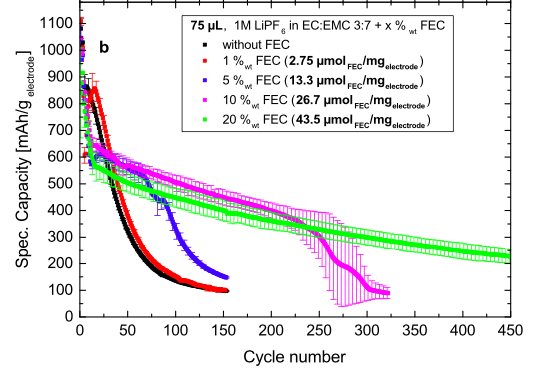
\includegraphics[scale=0.5]{images/Jung_et_al_Figure1b.png}
}

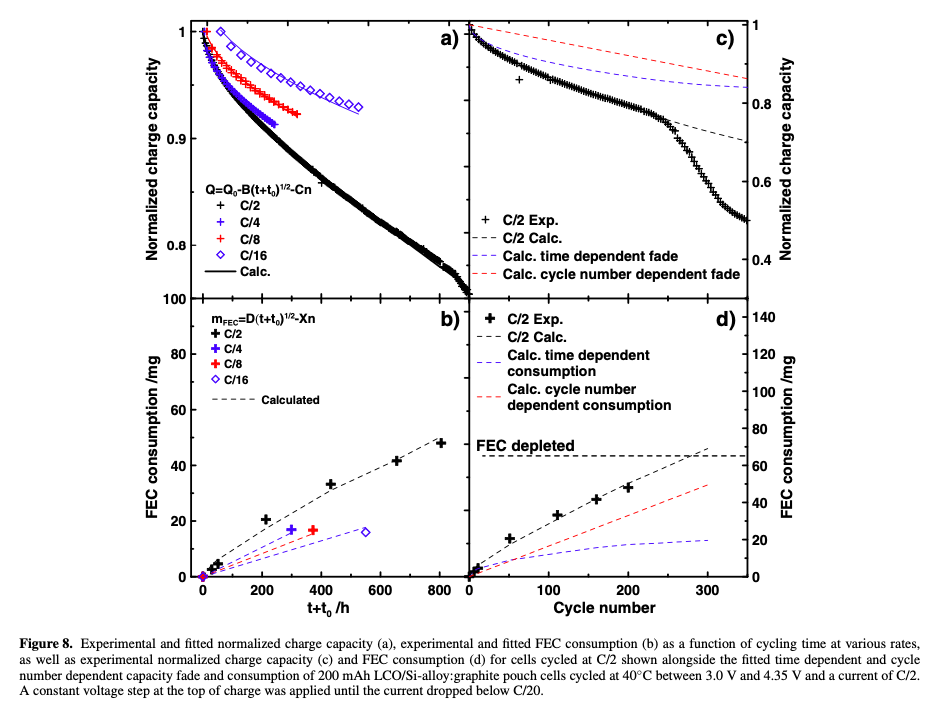
\includegraphics[scale=0.45]{images/Petibon_et_al_Figure8.png}

This knee pathway has a number of interesting implications.
First, since laboratory-built cells are often filled with high electrolyte volumes, knee mechanisms that are not present in lab testing may manifest in more commercially representative form factors.
As Wetjen et al.\cite{wetjen_differentiating_2017} emphasize,
maintaining representative electrolyte volumes in lab-scale cells is critical for accurately capturing this knee pathway in production-scale cells.
Second, nominally identical cells, cycled identically, but with different initial FEC concentrations exhibited minute electrochemical differences before the knee.\cite{jung_consumption_2016}
Theoretically, only the FEC consumed in a given cycle manifests in the electrochemical signals from cycling (e.g., differential capacity or differnetial voltage analysis); the excess FEC is not electrochemically detectable as it does not participate in reactions with the electrode.
Since the \emph{remaining} FEC amount is the main determinant of cycle life in these cells, the knee point of cells exhibiting this mechanism is not predictable via standard electrochemical signals.
An interesting proposal for future work is to evaluate other nondestructive probes (e.g., electrochemical impedance spectroscopy\cite{zhang_identifying_2020}, acoustic signals\cite{knehr_understanding_2018}) that may be sensitive to FEC concentration in the electrolyte.

(Tino) Kupper et al.~\cite{kupper_end--life_2018} model what they call `sudden death' by introducing a percolation threshold in the activity-saturation relationship, which is linked to electrolyte dry-out.

\subsection{Mechanical degradation (Philipp, Tino, Anna)}

\paragraph{Pressure.} (Philipp)
pressure can be set and measured with pouch \cite{wunsch_investigation_2019} and prismatic cells\cite{cannarella_stress_2014} ,only measured on cylindrical \cite{willenberg_high-precision_2020}

High stack pressure can cause knee. High mechanical stress is not evenly distributed throughout the inside of the pouch, causing heterogeneous delamination, surface film formation, and uneven lithium distribution. LAM attributed to anode from half-cell data, no change in LAM PE. There's a sweet spot for stack pressure, just like temperature.\cite{cannarella_stress_2014}

Pressure evolution different for different kinds of bracing (Wünsch et al.) Thickness increase for unbraced cells correlated with knee point. Lifetime can be increased from 500 to 3200 cycles with the right bracing. (Wünsch et al.)

CT study on 18650s reveals jelly roll deformation, pfang et al. \cite{pfrang_long-term_2018} using cells from Ecker et al. \cite{ecker_calendar_2014}
Pressure can enhance conductivity and particle link, and heterogenous pressure induces uneven ageing for example due to ageing \cite{bach_nonlinear_2016}

The effects discussed here are inherently multidimensional (at the macroscale) in nature and hence cannot be captured by standard electrochemical models, which are one-dimensional at the macroscale. Instead, they would require complex three-dimensional models, whose computational complexity is prohibitively high for simulating degradation over hundreds of cycles. We are not aware of any current modeling efforts in this direction [right?]. One reduced-order modeling approach could be to couple one-dimensional electrochemical models with network models for the jellyroll [cite Tranter].

\paragraph{Interaction of SEI growth with mechanical effects.} (Tino) [NEED TO CHECK HOW THIS IS DIFFERENT TO THE LAM SECTION IN PLATING]
Another possible mechanism that leads to a kneepoint is the accelerating SEI growth due to mechanical effects (stress and/or loss of active material).

This can occur, and be simulated, in various forms.
Laresgoiti et al.~\cite{laresgoiti_modeling_2015} introduce a fatigue model for loss of active material due to stress. They further show that particle volume changes lead to cracking of the SEI, which then exposes fresh particle surface causing accelerated SEI formation. Kupper et al.~\cite{kupper_end--life_2018} include this effect in a degradation model by directly including an empirical dependence on the tangential stress on the SEI layer into the SEI reaction term. In fact, as shown by Reniers et al.~\cite{reniers_review_2019}, even coupling Laresgoiti's model with a stress model (ignoring SEI growth) would lead to an accelerating growth rate since there is a positive feedback loop between higher stress and higher loss of active material.

A significantly different mechanism is proposed by Lin et al.~\cite{lin_comprehensive_2013}, who propose a mechanism whereby a combination of loss of lithium inventory (due to SEI reaction) and loss of active material in the positive electrode (due to Manganese dissolution) lead to a shift in the stoichiometry windows, which eventually accelerates the SEI reaction causing a knee point.
Jana et al.~\cite{jana_physical_2019} also include both SEI formation and loss of active material in their model, and have knee point effects that they attribute to `mechanical effects', but do not propose a model for how LAM contributes to these mechanical effects and instead leave them as `unmodeled'.
Check Dubarry's Cn/Cp argument.
Check Keil.

Nice figures for this in Kupper 2018, Louli 2019.

\section{Conclusions and future work}

\bibliographystyle{myIEEEtran}
\bibliography{refs_zotero}

Supporting Information

Table 1. Summary of experimental conditions leading to knee point

Yuliya: See table in Excel document tab 'SI-Exp Tables'. The content is there, but I'm still trying to figure out how to transfer it to Overleaf. Given that tables are difficult in Overleaf, I might not spend the time formatting it if we're just going to submit a Word document anyway. 


\end{document}
